%!TEX root = ../main.tex
\section{Designing a controller}
\label{sec:controller}

To control the speed of the DC motor a controller will have to be implemented to the system. A Simulink block diagram of the DC motor in figure~\ref{fig:dcmotormodel} is shown in figure~\ref{fig:dcblock}. From the block diagram the transfer function $P(s)$ of the motor can be derived as seen in equation~\ref{eq:fullplant}. $P(s)$ is rearranged to coincide with the form in equation~\ref{eq:simpleplant}. 
\begin{figure}[!h]
	\centering
	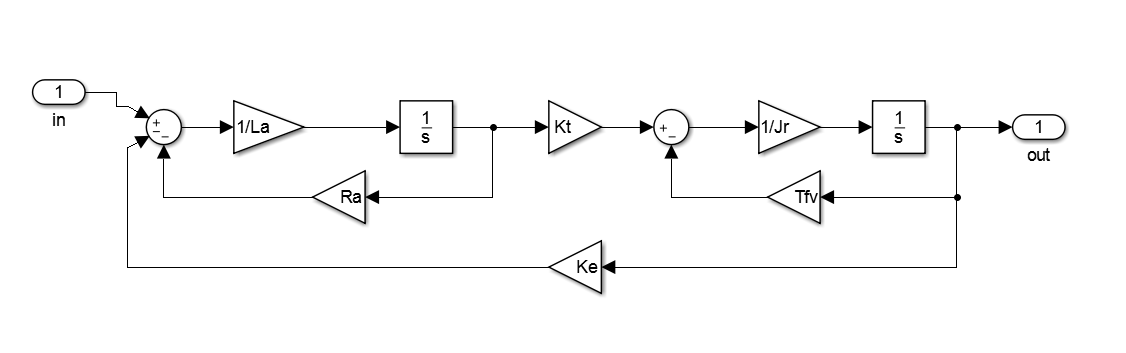
\includegraphics[width=1\linewidth]{graphics/dcblockdiagram}
	\caption{A Simulink block diagram of the full order DC motor.}
	\label{fig:dcblock}
\end{figure}


\begin{equation}
\label{eq:fullplant}
P(s) = \dfrac{\dfrac{K_m}{J_r L_a}}{s^2 + \dfrac{J_r R_a + L_a T_{fv}}{J_r L_a}s + \dfrac{R_a T_{fv} +K_m^2}{J_r L_a}}
\end{equation}

\begin{equation}
\label{eq:simpleplant}
P(s) = \dfrac{b_0}{s^2 + a_1 s + a_0}
\end{equation}


\subsection{PID controller}
 A commonly used controller is the PID controller~\cite{feedback}. 
 The name comes from its three adjustable parameters, the proportional gain $K_{P}$, integral gain $K_{I}$ and the derivative gain $K_{D}$. 
 The reason for its popularity is the wide range of operating conditions as well as being relatively easy to understand. 
 
 The controller is placed at the input of the motor, monitoring the output through a feedback. 
 The system is shown in figure~\ref{fig:pidcontrolsystem} where the plant is the DC motor. 
 The transfer function $H(s)$ of the system is shown in equation~\ref{eq:tfpidsystem} where $C(s)$ is the transfer function of the controller.

\begin{figure}[!h]
	\centering
	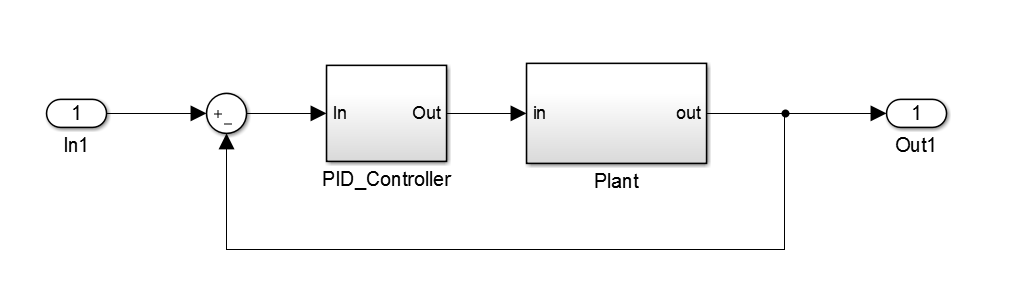
\includegraphics[width=.75\linewidth]{graphics/controlsystem}
	\caption{Block diagram of the PID control system. The plant represents the DC motor.}
	\label{fig:pidcontrolsystem}	
\end{figure}

\begin{equation}
\label{eq:tfpidsystem}
H(s) = \dfrac{C(s)P(s)}{1+C(s)P(s)}
\end{equation}

A block diagram for the PID controller can be seen in figure~\ref{fig:pidblock} and its transfer function in equation~\ref{eq:pid}.  

\begin{figure}[!h]
	\centering
	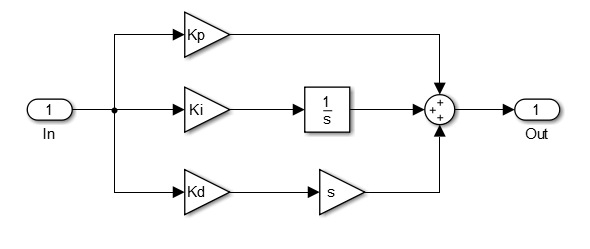
\includegraphics[width=.7\linewidth]{graphics/pidcontroller}
	\caption{Block diagram of the PID-controller}
	\label{fig:pidblock}
\end{figure}

\begin{equation}
\label{eq:pid}
C(s) = K_P + \dfrac{K_I}{s} +K_D s
\end{equation}

Inserting the transfer functions $C(s)$ and $P(S)$ into the transfer function $H(s)$ and rearranging it, $H(s)$ becomes equation~\ref{eq:pidfulltf}. On this form, the denominator describes the poles of the system. The denominator is the system's characteristic equation.

\begin{equation}
\label{eq:pidfulltf}
H(s) = \dfrac{b_0 (K_D s^2 + K_P s K_I)}{s^3 + (a_1 + b_0 K_D)s^2 (a_0 + b_0 K_P)s + b_0 K_I }
\end{equation}


\subsection{IPD controller}
An equivalent setup to the PID controller is the IPD controller, which does not introduce zeros to the system. It still uses the same gains, proportional, integral and derivative.

\begin{figure}[!h]
	\centering
	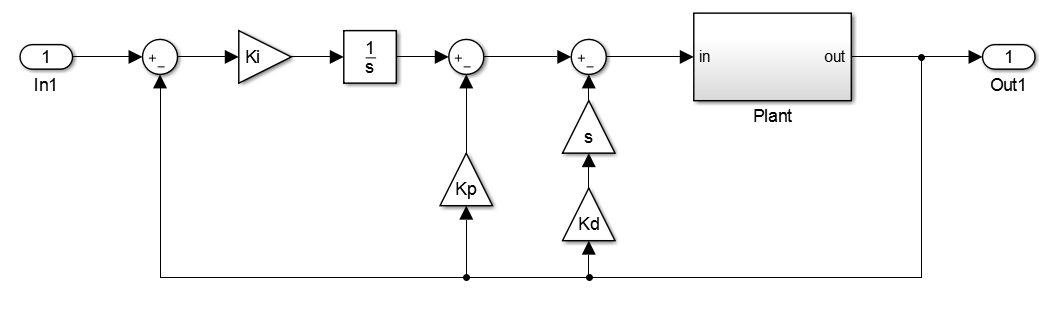
\includegraphics[width=1\linewidth]{graphics/ipdcontroller}
	\caption{Block diagram of the IPD control setup}
	\label{fig:ipdcontrolsystem}	
\end{figure}

The transfer function of the IPD controller system becomes as seen in equation~\ref{eq:tfipdsystem}. The transfer functions $P(s)$ and $C(s)$ are the same as in equation~\ref{eq:tfpidsystem}. It is noticed that the transfer function indeed introduces no zeros to the system.

\begin{equation}
\label{eq:tfipdsystem}
H(s) = \dfrac{\dfrac{K_I}{s} P(s)}{1+C(s)P(s)}
\end{equation}

With insertion and rearranging, the transfer function $H(s)$ takes the form of equation~\ref{eq:ipdfulltf}. Now it can be seen that indeed the IPD controller does not introduce any zeros to the system and the characteristic equation is the same as the one for the PID controller. Thus the same controller gains can be used in both cases.

\begin{equation}
\label{eq:ipdfulltf}
H(s) = \dfrac{b_0 K_I}{s^3 + (a_1 + b_0 K_D)s^2 (a_0 + b_0 K_P)s + b_0 K_I }
\end{equation}

\subsection{Noise Filtering}

The derivative part of the PID controller will resist any sudden change in the system. This is what helps the system stop oscillating. However, when noise is introduced into the system, the derivative term acts on the fast, sudden change and can destabilize the system. In other words, the derivative term can and will increase the noise. For this reason a low pass filter is needed on the derivative path. This is done with changing $s$ on the derivative gain to $N/(s + N)$ where $N$ is $1/T_f$ and $T_f$ is the filter time constant and N is the cut off frequency. The block diagram for the controllers then become as seen in figures~\ref{fig:pidfilter} and~\ref{fig:ipdfilter} respectively.

\begin{figure}[!h]
	\centering
	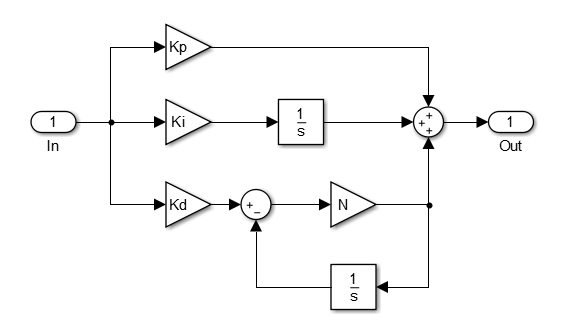
\includegraphics[width=.7\linewidth]{graphics/pidwfilter}
	\caption{Block diagram of the PID controller with filter}
	\label{fig:pidfilter}
\end{figure}

\begin{figure}[!h]
	\centering
	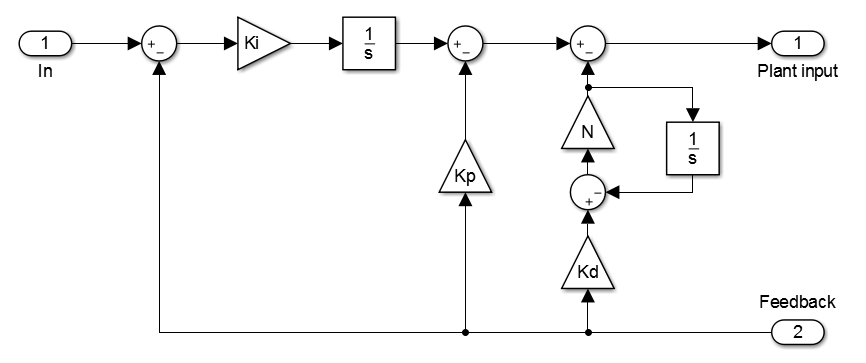
\includegraphics[width=.9\linewidth]{graphics/ipdwfilter}
	\caption{Block diagram of the IPD controller with filter}
	\label{fig:ipdfilter}
\end{figure}


\subsection{Anti-Windup Design}
\todo{Explanation of the appearance of the nonlinear region-Erlingur}
During the function of the controller, there is a possibility that it will operate in a nonlinear region where increasing the control signal has no effect on the system output. 
This introduces time delay to the response of the system, thus reducing its overall performance. 
This behaviour can be counteracted using an anti-windup strategy such as the one in figure~\ref{fig:ipdantiwindupstrategy}.

\begin{figure}[!h]
	\centering
	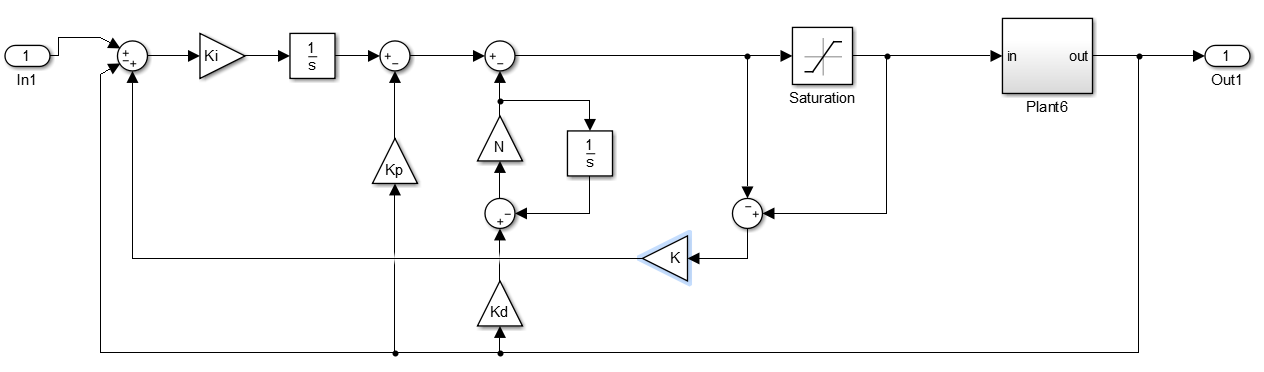
\includegraphics[width=1\linewidth]{graphics/ipdwindupdesign}
	\caption{Block diagram of the IPD controller with anti-windup design}
	\label{fig:ipdantiwindupstrategy}
\end{figure}

As figure~\ref{fig:antiwindupresponses} shows, using this strategy eliminates the overshoot of the system. The gain $K$ is the one that determines that behaviour and can be chosen doing experiments using trial and error. An interesting observation is that the value of $K$ for the PID controller is quite different from the one for the IPD controller. Specifically, a suitable value for PID is $K=10$, while for IPD is $K=10000$. That conclusion has been reached through experiments, and the results can be seen in figure~\ref{fig:pidwindupvaluecomp}.

\begin{figure}
	\centering
	\begin{subfigure}[b]{0.45\textwidth}
		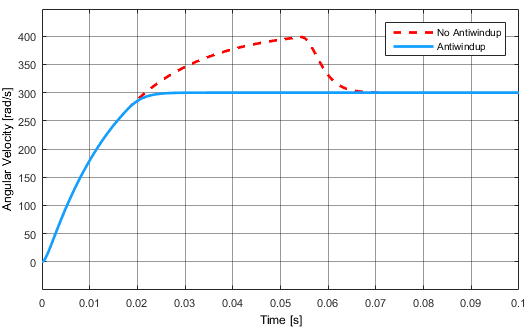
\includegraphics[width=\textwidth]{graphics/pidwindupresponse}
		\caption{PID controller.}
		\label{fig:pidwindupresponse}
	\end{subfigure}
	~ %add desired spacing between images, e. g. ~, \quad, \qquad, \hfill etc. 
	%(or a blank line to force the subfigure onto a new line)
	\begin{subfigure}[b]{0.45\textwidth}
		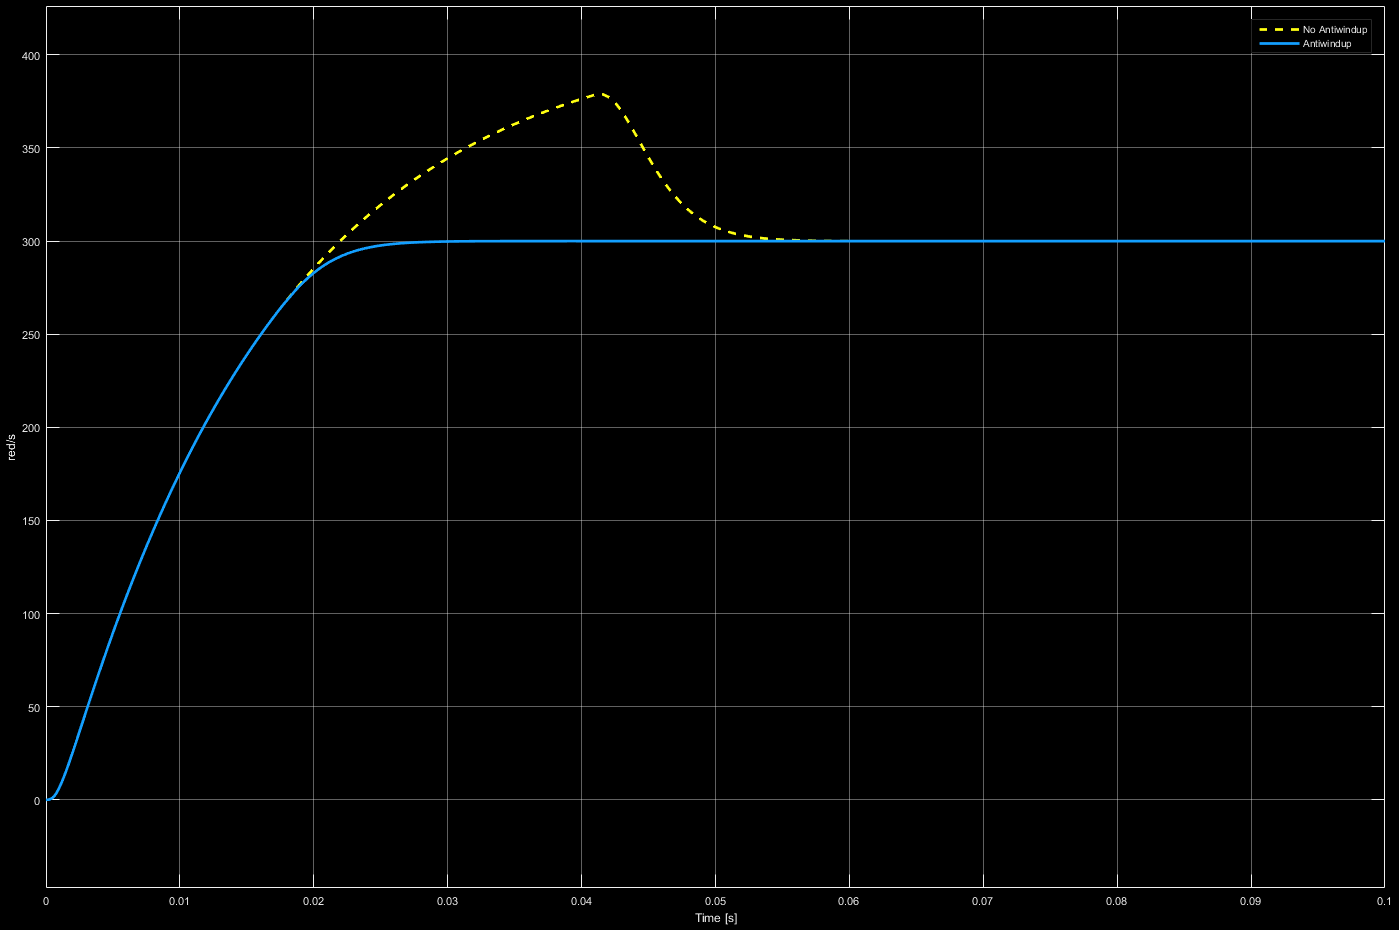
\includegraphics[width=\textwidth]{graphics/ipdwindupresponse}
		\caption{IPD controller.}
		\label{fig:ipdwindupresponse}
	\end{subfigure}
	\caption{Responses of controllers without and with anti-windup design.}\label{fig:antiwindupresponses}
\end{figure}

\begin{figure}[!h]
	\centering
	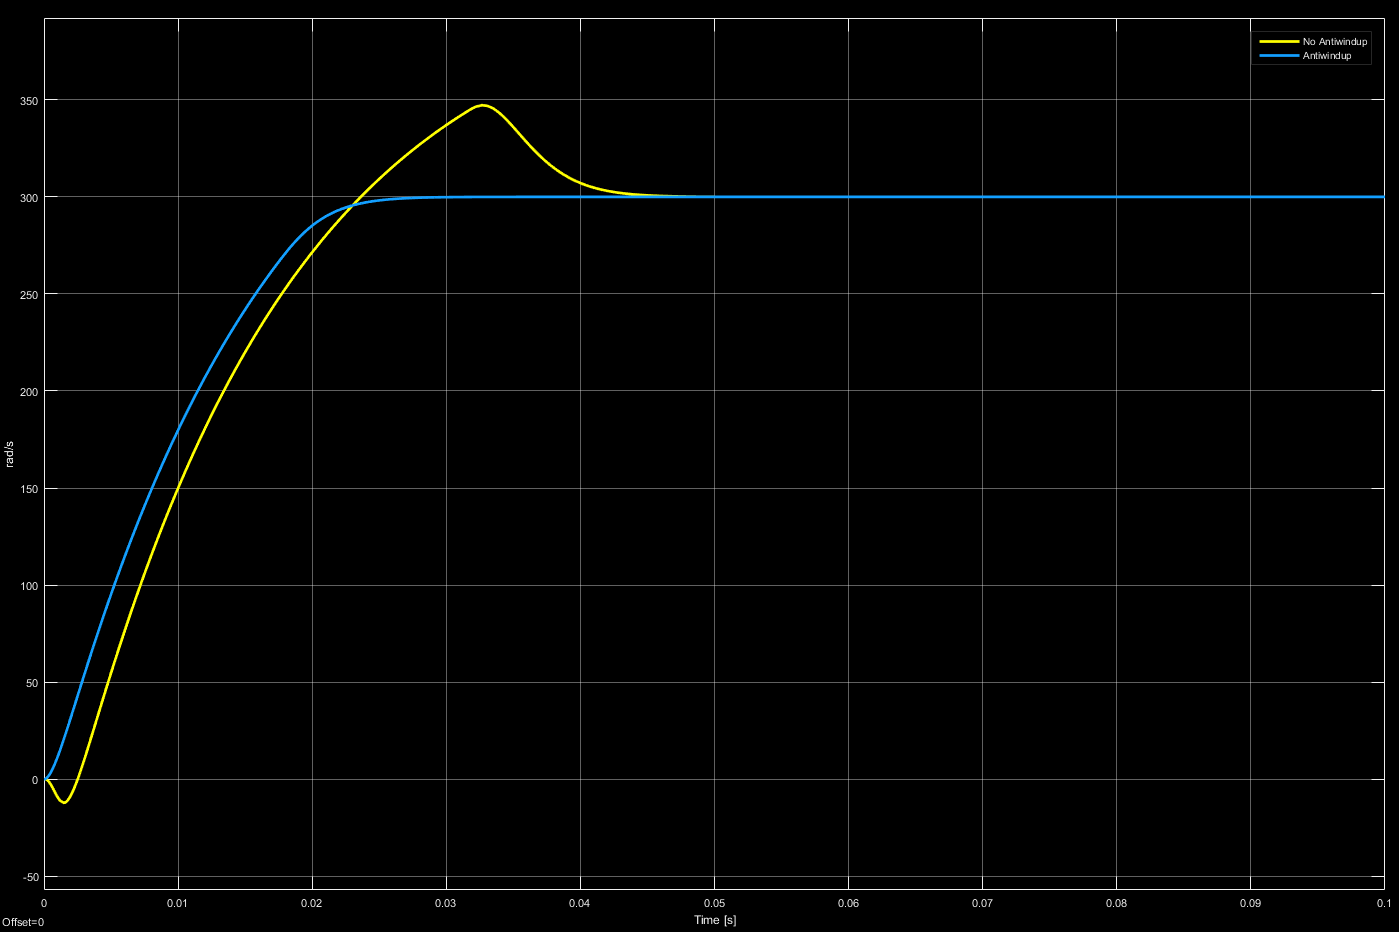
\includegraphics[width=.6\linewidth]{graphics/pidwindupvaluecomp}
	\caption[PID behaviour with different anti-windup gain.]{PID behaviour with different anti-windup gain. The higher gain being 10000 while the lower is 10.}
	\label{fig:pidwindupvaluecomp}
\end{figure}

\subsection{Controller Gain Design}
The controller gains are then to be designed. To achieve that the settling time method is introduced.


\subsubsection{Settling Time Formula}

The equation~\ref{eq:settling} is used for the system's desired response to enter the 5$\%$ error band within a specified settling time of $T_s$ and $n$ being the order of the controller.
\begin{equation}
\centering
\label{eq:settling}
\alpha = \dfrac{1.5(1 + n)}{T_s}
\end{equation}

\begin{table}[!h]
	\caption{ Coefficients of
		closed loop differential
		equation based on settling
		time formula~\cite{feedback}}
	\centering
	\begin{tabular}{|c|c|c|c|}
		\hline
		n & 2 & 3 & 4\\
		\hline
		$d_0$ & $\alpha^2$ & $\alpha^3$ & $\alpha^4$\\ 
		$d_1$ & $2\alpha$ & $3\alpha^2$ & $4\alpha^3$\\
		$d_2$ & - & $3\alpha$ & $6\alpha^2$\\
		$d_0$ & - & - & $4\alpha$\\
		\hline	
		
	\end{tabular}
	\label{table:coefsettlingtime}
\end{table}


\subsubsection{Full Order Systems}

As the equations~\ref{eq:pidfulltf} and~\ref{eq:ipdfulltf} show, their denominator is in the standard form of equation~\ref{eq:stdchararacteristic}. To calculate the controller gains the characteristic equation is compared to the coefficients in table~\ref{table:coefsettlingtime} where the order of the system in this case is $n=3$. The gain equations for $K_I, K_P$ and $K_D$ can be seen in equations~\ref{eq:pidki},~\ref{eq:pidkp} and~\ref{eq:pidkd} respectively. 


\begin{equation}
\centering
\label{eq:stdchararacteristic}
s^n + d_{n-1}s^{n-1} + \cdots + d_1 s + d_0 
\end{equation}

\begin{align}
\label{eq:pidki}
d_0 &= b_0 K_I = \alpha^3
\\
\label{eq:pidkp}
d_1 &= a_0 + b_0 K_P = 3\alpha^2
\\
\label{eq:pidkd}
d_2 &= a_1 + b_0 K_D = 3\alpha
\end{align}

Solving the above equations using the parameters and $T_s$ = 10~ms, the gains receive the values:
\begin{align*}
K_I &= 62.3855
\\
K_P &= 0.2752
\\
K_D &= 1.7910\cdot10^{-4}
\end{align*}

And again for a settling time $T_s$ = 100~ms

\begin{align*}
K_I &= 0.0945
\\
K_P &= -0.0315
\\
K_D &= -5.3532\cdot10^{-4}
\end{align*}


\subsubsection{Reduced Order Systems}
\todo[inline]{We should tell why we can reduce the order. Maybe a pole zero plot -Erlingur}
In the case of a reduced order system, the controller derivative's gain is equal to zero and the inductance of the motor $L_a$ is not taken into account during the calculations. The reduced transfer function takes the form of equation~\ref{eq:pireducedtf}.

\begin{equation}
\label{eq:pireducedtf}
H(s) = \dfrac{b_0(K_Ps + K_I)}{s^2 + (a_0 + b_0 K_P)s + b_0 K_I }
\end{equation}

Matching the characteristic equation with the standard form and looking at the coefficients in table~\ref{table:coefsettlingtime}, the equations for the controller gains, $K_i$ and $K_p$ become as seen in equations~\ref{eq:piki} and~\ref{eq:pikp} respectively.

\begin{align}
\label{eq:piki}
d_0 &= b_0 K_I = \alpha^2
\\
\label{eq:pikp}
d_1 &= a_0 + b_0 K_P = 2\alpha
\end{align}

Similarly, using the parameters and $T_s=10ms$, the gains in this case are:

\begin{align*}
K_I &= 221
\\
K_P &= 0.7
\end{align*}
 
 and again for the settling time of $T_s$ = 100ms:
 
 \begin{align*}
 K_I &= 2.2101
 \\
 K_P &= 0.0374
 \end{align*}
 